\chapter{Cálculo diferencial}

\setcounter{section}{3}
\section{Derivada de una función}

\begin{tcolorbox}
    \begin{def.}[Definición de derivada]
	La derivada $f'(x)$ está definida por la igualdad 
	$$f'(x)=\lim_{h\to 0}\dfrac{f(x+h)-f(x)}{h},$$
	siempre que exista el límite. El número $f'(x)$ también se denomina coeficiente de variación de $f$ en $x$.
    \end{def.}
\end{tcolorbox}
\vspace{.7cm}

\begin{ejem}[Derivada de una función potencial de exponente entero positivo]
    Consideremos el caso $f(x)=x^n$, siendo $n$ un entero positivo. El cociente de diferencias es ahora\\
    $$\dfrac{f(x+h)-f(x)}{h}=\dfrac{(x+h)^n-x^n}{h}$$\\
    Para estudiar este cociente al tender $h$ a cero, podemos proceder de dos maneras, o por la descomposición factorial del numerador considerado como diferencia de dos potencias n-simas o aplicando el teorema del binomio para el desarrollo de $(x + h)^n$. Seguiremos con el primer método.\\

    En álgebra elemental se tiene la identidad
    $$a^n - b^n = (b-a)\sum_{k=0}^{n-1} a^k b^{n-1-k}$$
    Si se toma $a=x+h$ y $b=x$ y dividimos ambos miembros por $h$, esa identidad se transforma en \\
    $$\dfrac{(x+h)^n-x^n}{h} = \sum_{k=0}^{n-1}(x+h)^k x^{n-1-k}$$\\
    En la suma hay $n$ términos. Cuando $h$ tiende a $0$, $(x+h)^k$ tiende a $x^k$, el k-ésimo término tiende a $x^k x^{n-1-k}=x^{n-1},$ y por tanto la suma de los $n$ términos tiende a $nx^{n-1}$. De esto resulta que \\
    $$f'(x)=nx^{n-1}\quad \forall \; x.$$\\
\end{ejem}

\begin{ejem}[Derivada de la función seno]
    Sea $s(x)=\sen x$. El cociente de diferencias es
    $$\dfrac{s(x+h)-s(x)}{h}=\dfrac{\sen(x+h)-\sen x}{h}$$
    Para transformarlo de modo que haga posible calcular el límite cuando $h\to 0$, utilizamos la identidad trigonométrica
    $$\sen y -\sen x = 2\sen \dfrac{y-x}{2}\cos \dfrac{y+x}{2}$$
    poniendo $y=x+h$. Esto conduce a la fórmula
    $$\dfrac{\sen(x+h)-\sen x}{h}=\dfrac{\sen\frac{h}{2}}{\frac{h}{2}} \cos \left(x+\dfrac{h}{2}\right)$$
    Como $h\to 0$, el factor $\cos(x+\frac{1}{2}h)\to \cos x$ por la continuidad del coseno. Así mismo, la fórmula 
    $$\lim_{x\to 0}\dfrac{\sen x}{x}=1,$$
    demuestra que
    $$\dfrac{\sen \frac{h}{2}}{\frac{h}{2}}\to 1\;\mbox{ para todo } \; h\to 0$$
    Por lo tanto el cociente de diferencias tiene como límite $\cos x$ cuando $h\to 0$. Dicho de otro modo, $s'(x)=\cos x;$ para todo $x$; la derivada de la función seno es la función coseno.\\\\ 
\end{ejem}

\begin{ejem}[Derivada de la función coseno]
    Sea $c(x)=\cos x$. Demostraremos que $c'(x)=-\sen x$; esto es, la derivada de la función coseno es menos la función seno. Partamos de la identidad
    $$\cos y - \cos x = -2\sen \dfrac{y-x}{2}\sen \dfrac{y+x}{2}$$
    y pongamos $y=x+h$. Esto nos conduce a la fórmula
    $$\dfrac{\cos(x+h)-\cos x}{h}=-\dfrac{\sen \frac{h}{2}}{\frac{h}{2}}\sen \left(x+\dfrac{h}{2}\right).$$
    La continuidad del seno demuestra que $\left(x+\frac{1}{2}h\right)\to x$ cuando $h\to 0$; luego ya que 
    $$\dfrac{\sen \frac{h}{2}}{\frac{h}{2}}\to 1\;\mbox{ para todo } \; h\to 0$$
    obtenemos $c'(x)=-\sen x$.\\
\end{ejem}

\begin{ejem}[Derivada de la función raíz n-esima]
    Si $n$ es un entero positivo, sea $f(x)=x^{1/n}$ para $x>0$. El cociente de diferencias para $f$ es
    $$\dfrac{f(x+h)-f(x)}{h}=\dfrac{(x+h)^{1/n}-x^{1/n}}{h}.$$
    Pongamos $u=(x+h)^{1/n}$ y $v=x^{1/n}$. Tenemos entonces $u^n = x+h$ y $v^n=x,$ con lo que $h=u^n-v^n$, y el cociente de diferencias toma la forma
    $$\dfrac{f(x+h)-f(x)}{h}=\dfrac{u-v}{u^n -v^n}=\dfrac{1}{u^{n-1}+u^{n-2}v + \ldots + uv^{n-2}v^{n-1}}$$
    La continuidad de la función raíz n-sima prueba que $u \to v$ cuando $h \to O$. Por consiguiente cada término del denominador del miembro de la derecha tiene límite $v^{n-1}$ cuando $h \to O$. En total hay $n$ términos, con lo que el cociente de diferencias tiene como límite $v^{1-n}/n$. Puesto que  $v = x^{1/n}$, esto demuestra que
    $$f'(x)=\dfrac{1}{n}x^{1/n-1}.$$\\
\end{ejem}

\begin{tcolorbox}
    \begin{ejem}[Continuidad de las funciones que admiten derivada]
	Si una función $f$ tiene derivada en un punto $x$, es también continua en $x$. Para demostrar, empleamos la identidad
	$$f(x+h)=f(x)+h\left(\dfrac{f(x+h)-f(x)}{h}\right)$$
	que es válida para $h\neq 0$. Si hacemos que $h\to 0$, el cociente de diferencias del segundo miembro tiende a $f'(x)$, puesto que este cociente está multiplicando por un factor que tiende a $0$, el segundo término del segundo miembro tiende a $0\cdot f'(x)$. Esto demuestra que $f(x+h)\to f(x)$ cuando $h\to 0$ y por tanto que $f$ es continua en $x$.
    \end{ejem}
\end{tcolorbox}

\section{Álgebra de las derivadas}

\begin{teo}
    Sean $f$ y $g$ dos funciones definidas en un intervalo común. En cada punto en que $f$ y $g$ tienen derivadas, también las tienen la suma $f+g$, la diferencia $f-g$, el producto $f\cdot g$ y el cociente $f/g$. (Para $f/g$ hay que añadir también que $g$ ha de ser distinta de cero en el punto considerado). Las derivadas de estas funciones están dadas por las siguientes fórmulas:
    \begin{enumerate}[(i)]
	\item $(f+g)' = f'+g',$
	\item $(f-g)' = f'-g',$
	\item $(f\cdot g)'=f\cdot g' + g\cdot f',$
	\item $\left(\dfrac{f}{g}\right)' = \dfrac{g\cdot f' - f\cdot g'}{g^2}$ en puntos $x$ donde $g(x)\neq 0$.\\\\
    \end{enumerate}
	Demostración.-\; Demostración de (i). Sea $x$ un punto en el que existen ambas derivadas $f'(x)$ y $g'(x)$: El cociente de diferencias para $f+g$ es
	$$\dfrac{(f+g)(x+h)-(f+g)(x)}{h}=\dfrac{[f(x+h)+g(x+h)]-[f(x)+g(x)]}{h}=\dfrac{f(x+h)-f(x)}{h}+\dfrac{g(x+h)-g(x)}{h}$$
	Cuando $h\to 0$, el primer cociente del segundo miembro tiende a $f'(x)$ y el segundo a $g'(x)$ y por tanto la suma tiende a $f'(x)+g'(x)$. La demostración de (ii) es análoga.\\

	Demostración de (iii). El cociente de diferencias para el producto $f\cdot g$ es:
	$$\dfrac{f(x+h)g(x+h)-f(x)g(x)}{h}.$$
	Para estudiar este cociente cuando $h\to 0$ se suma y resta al numerador un término conveniente para que se puede escribir la fórmula dada como la suma de dos términos en los que aparezca los cocientes de diferencias de $f$ y $g$. Sumando y restando $f(x)f(x+h)$ se convierte en
	$$\dfrac{f(x+h)g(x+h)-f(x)g(x)}{h}=g(x)\dfrac{f(x+h)-f(x)}{h}+f(x+h)\dfrac{g(x+h)-g(x)}{h}.$$
	Cuando $h\to 0$ el primer término del segundo miembro tiende a $g(x)f'(x)$, y puesto que $f(x+h)\to f(x),$ el segundo término tiende a $f(x)g'(x)$, lo que demuestra (iii).\\

	Demostración de (iv). Un caso particular de (iv) se tiene cuando $f(x)=1$ para todo $x$. En este caso $f'(x)=0$ y (iv) se reduce a la fórmula
	$$\left(\dfrac{1}{g}\right)'=-\dfrac{g'}{g^2}$$
	suponiendo que $f(x)\neq 0$ partir de este caso particular, se puede deducir la fórmula general (iv) escribiendo $f/g$ como producto y aplicando (iii), con lo cual se tiene:
	$$\left(f\cdot \dfrac{1}{g}\right)'=\dfrac{1}{g}\cdot f' + f\cdot \left(\dfrac{1}{g}\right)'=\dfrac{f'}{g}-\dfrac{f\cdot g'}{g^2}=\dfrac{g\cdot f'-f\cdot g'}{g^2}$$
	Por tanto, queda solamente por probar $\left(\dfrac{1}{g}\right)'=-\dfrac{g'}{g^2}$. El cociente de diferencias de $1/g$ es:
	$$\dfrac{\frac{1}{g(x+h)}-\frac{1}{g(x)}}{h} = -\dfrac{g(x+h)-g(x)}{h}\cdot \dfrac{1}{g(x)}\dfrac{1}{g(x+h)}$$
	Cuando $h\to 0,$ el primer cociente de la derecha tiende a $g'(x)$ y el tercer factor tiende a $\frac{1}{g(x)}$. Se requiere la continuidad de $g$ en $x$ ya que se hace uso del hecho que $g(x+h)\to g(x)$ cuando $h\to 0$. Por tanto, el cociente tiende a $-\dfrac{g'(x)}{g(x)^2}$.\\\\

\end{teo}

Un caso particular de (iii) se tiene cuando una de las dos funciones es constante, por ejemplo, $g(x) = c$ para todo valor de $x$. En este caso, (iii) se transforma en: $(c \cdot f)' = c\cdot f'$; es decir, la derivada del producto de una función por una constante es el producto de la derivada de la función por la constante. Combinando esta propiedad con la de la derivada de una suma [propiedad (i)] se tiene, que para cada par de constantes $c_1$ y $c_2$, es:
$$(c_1f+c_2g)'=c_1f'+c_2g'$$
Esta propiedad se denomina propiedad lineal de la derivada, y es análoga a la propiedad lineal de la integral.\\
Aplicando el método de inducción se puede extender la propiedad lineal a un número cualquiera finito de sumandos:
$$\left(\sum_{i=1}^n c_i\cdot f_i\right)' = \sum_{i=1}^n c_i\cdot f_i',$$
donde $c_1, c_2, c_3,\ldots , c_n$ son constantes y $f_1, f_2, \ldots , f_n$ son funciones cuyas derivadas son $f_1',f_2',\ldots, f_n'$.\\
Cuando se consideran los valores de estas funciones en un punto x, se obtienen fórmulas entre números; así la fórmula (i) implica
$$(f+g)(x)=f'(x)+g'(x)$$

\begin{ejem}[funciones Racionales]
    Si $r$ es el cociente de dos polinomios, es decir, $r(x)=p(x)/q(x)$, la derivada $r'(x)$ se puede calcular por medio de la fórmula del cociente (iv) del teorema 4.1. La derivada existe para todo $x$ en el que $g(x)\neq 0$. Obsérvese que la función $r'$ así definida es a su vez una función racional. En particular, si $r(x)=1/x^m$ donde $m$ es un entero positivo y $x\neq 0$ se tiene:
    $$r'(x)=\dfrac{x^m\cdot 0 - mx^{m-1}}{x^{2m}}=\dfrac{-m}{x^{m+1}}$$
    Escribiendo este resultado en la forma: $r'(x) = - mx^{-m-1}$ se obtiene una extensión a exponentes negativos de la fórmula dada para la derivación de potencias n-simas para $n$ positivo.\\\\
\end{ejem}

\section{Ejercicios}

\begin{enumerate}[\bfseries 1.]

    %--------------------1.
    \item Si $f(x)=2+x-x^2$, calcular $f'(0),f'(\frac{1}{2}),f'(1),f'(-10)$.\\\\
	Respuesta.-\; Por definición sea,
	$$\begin{array}{rcl}
	    f'(x)&=&\lim\limits_{h\to 0}\dfrac{\left[2+(x+h)-(x+h)^2\right]-(2+x-x^2)}{h}\\\\
		 &=&\lim\limits_{h\to 0}\dfrac{2+x+h-x^2-2xh-h^2-2-x+x^2}{h}\\\\
		 &=&\lim\limits_{h\to 0} \dfrac{h(1-2x-h)}{h}\\\\
		 &=&1-2x\\\\
	\end{array}$$
	De donde 
	$$\begin{array}{rclcr}
	    f'(0)&=&1-2\cdot 0 &=&1\\\\
	    f'(\frac{1}{2})&=&1-2\cdot\frac{1}{2} &=& 0\\\\
	    f'(1)&=&1-2\cdot 1 &=& -1\\\\
	    f'(-10)&=&1-2\cdot (-10) &=& 21\\\\
	\end{array}$$
	\vspace{.7cm}

    %--------------------2.
    \item Si $f(x)=\frac{1}{3}x^3+\frac{1}{2}x^2-2x$, encontrar todos los valores de $x$ para los que \\
	\begin{enumerate}[(a)]

	    %---------- (a)
	    \item $f'(x)=0.$\\\\
		Respuesta.-\; Sea $f'(x)=x^2+x-2$, entonces 
		$$x^2+x-2=0\quad \Rightarrow \quad x_1=1\quad \mbox{y} \quad x_2=-2.$$\\

	    %---------- (b)
	    \item $f'(x)=-2$.\\\\
		Respuesta.-\;  Sea $f'(x)=x^2+x-2$, entonces
		$$x^2+x-2=-2\quad \Rightarrow \quad x^2+x = 0  \quad \Rightarrow \quad x_1=0 \quad \mbox{y} \quad x_2=-1.$$\\

	    %---------- (c)
	    \item $f'(x)=10$.\\\\
		Respuesta.-\; Sea $f'(x)=x^2+x-2$, entonces
		$$x^2+x-2=10\quad \Rightarrow \quad x^2+x -12 = 0  \quad \Rightarrow \quad x_1=3 \quad \mbox{y} \quad x_2=-4.$$\\\\

	\end{enumerate}

    En los ejercicios del 3 al 12, obtener una fórmula para $f'(x)$ si $f(x)$ es la que se indica.\\\\

    %--------------------3.
    \item $f(x)=x^2+2x+2$.\\\\
	Respuesta.-\; Por definición,
	$$\begin{array}{rcl}
	    f'(x)&=&\lim\limits_{h\to 0}\dfrac{(x+h)^2+2(x+h)+2-(x^2+2x+2)}{h}\\\\
		 &=&\lim\limits_{h\to 0}\dfrac{x^2+2xh+h^2+2x+2h+2-x^2-2x-2}{h}\\\\
		 &=&\lim\limits_{h\to 0}\dfrac{h^2+2xh+2h}{h}\\\\
		 &=&\lim\limits_{h\to 0}\dfrac{h(h+2x+2)}{h}\\\\
		 &=&2x+2\\\\
	\end{array}$$

    %--------------------4.
    \item $f(x)=x^4+\sen x$.\\\\
	Respuesta.-\; Ya que $(f+g)'=f'+g'$ y sabiendo que la derivada de $\sen x$ es $\cos x$, entonces
	$$f'(x) = 3x^2+\cos x.$$\\

    %--------------------5.
    \item $f(x)=x^4\sen x$.\\\\
	Respuesta.-\; Ya que $(fg)'=f\cdot g'+g\cdot f'$ y la derivada de $\sen x$ es $\cos x$, entonces
	$$f'(x) = x^4\cos x + 4x^3 \sen x.$$\\

    %--------------------6.
    \item $f(x)=\dfrac{1}{x+1},\quad x\neq -1.$\\\\
	Respuesta.-\; Sean $g(x)=1$ y $h(x)=x+1$. Sabemos que $\left(\dfrac{g}{h}\right)'=\dfrac{h\cdot g'-g\cdot h'}{h^2}$, entonces
	$$f'(x)=\dfrac{(x+1)\cdot 1' -1\cdot(x+1)'}{(x+1)^2}=\dfrac{1\cdot0 - 1\cdot 1}{(x+1)^2}=\dfrac{1}{(x+1)^2}.$$\\

    %--------------------7.
    \item $f(x)=\dfrac{1}{x^2+1}+x^5\cos x$.\\\\
	Respuesta.-\; Sean, $k(x)=1,\; g(x)=x^2+1,\; h(x)=x^5$ y $j(x)=\cos x$. Ya que $\left(\dfrac{k}{g}\right)'=\dfrac{g\cdot k'-k\cdot g'}{g^2}$, $(hj)'=h\cdot j'+j\cdot h'$ y la derivada de $\cos x$ es $-\sen x$, entonces 
	$$\begin{array}{rcl}
	    &=&\lim\limits_{h\to 0} \dfrac{(x^2+1)\cdot1'-1\cdot (x^2+1)'}{(x^2+1)^2}+x^5\cdot (\cos x)'+\cos x\cdot (x^5)'\\\\
	    &=&\lim\limits_{h\to 0}\dfrac{- 2x}{(x^2+1)^2}+x^5\cdot (-\sen x) + \cos x\cdot 5x^4\\\\
	\end{array}$$

    %--------------------8.
    \item $f(x)=\dfrac{x}{x-1},\quad x\neq 1$.\\\\
	Respuesta.-\; Sean $k(x)=x$ y $g(x)=x-1$. Ya que $\left(\dfrac{k}{g}\right)'=\dfrac{g\cdot k'-k\cdot g'}{g^2}$ para $g\neq 0$, entonces
	$$f'(x) = \dfrac{x-1 - x}{(x-1)^2} = -\dfrac{1}{(x-1)^2}.$$\\

    %--------------------9.
    \item $f(x)=\dfrac{1}{2+\cos x}.$\\\\
	Respuesta.-\; $$f'(x)=\dfrac{(2+\cos x)\cdot 0+\sen x}{(2+\cos x)^2}=\dfrac{\sen x}{(2+\cos x)^2}.$$\\

    %--------------------10.
    \item $f(x)=\dfrac{x^2+3x+2}{x^4+x^2+1}$.\\\\
	Respuesta.-\; $$f'(x)=\dfrac{(x^4+x^2+1)(2x+3)-(x^2+3x+2)(4x^3+2x)}{(x^4+x^2+1)^2} = \dfrac{2x^5+9x^4+8x^3+3x^2+2x-3}{(x^4+x^2+1)^2}.$$\\

    %--------------------11.
    \item $f(x)=\dfrac{2-\sen x}{2-\cos x}$.\\\\
	Respuesta.-\; $$\begin{array}{rcl}
	    f'(x)&=&\dfrac{(-\cos x)(2-\cos x)-(2-\sen x)(\sen x)}{(2-\cos x)^2}\\\\
		 &=&\dfrac{-2\cos x + \cos^2 x - 2\sen x +\sen^2 x}{(2-\cos x)^2}\\\\
		 &=&\dfrac{1-2(\sen x + \cos x)}{(2-\cos x)^2}
	\end{array}$$
	\vspace{.7cm}

    %--------------------12.
    \item $f(x)=\dfrac{x\sen x}{1+x^2}$.\\\\
	Respuesta.-\; Primero escribimos 
	$$f(x)=\dfrac{x\sen x}{1+x^2}=x\left(\dfrac{\sen x}{1+x^2}\right)$$
	Luego usando el la regla del producto y del cociente para derivadas tenemos,
	$$f'(x)=\dfrac{\sen x}{1+x^2}+x\left[\dfrac{(1+x^2)\cos x - 2x\sen x}{(1+x^2)^2}\right] =\dfrac{\sen x + x \cos x}{1+x^2}- \dfrac{2x^2\sen x}{(1+x^2)^2}.$$\\

    %--------------------13.
    \item Se supone que la altura $f(t)$ de un proyectil, $t$ segundos después de haber sido lanzado hacia arriba a partir del suelo con una velocidad inicial de $v_0$ metros por segundo, está dada por la fórmula:
	$$f(t)=v_0t-16t^2.$$

	\begin{enumerate}[(a)]

	    %---------- (a)
	    \item Aplíquese el método descrito en la Sección 4.2 para probar que la velocidad media del proyectil durante el intervalo de tiempo de $t$ a $t+h$ es $v_0-32t-16h$ pies sobre segundo, y que la velocidad instantánea en el instante $t$ es $v_0-32t$ pies por segundo.\\\\
		Respuesta.-\; La velocidad media es dada por,
		$$\dfrac{f(t+h)-f(t)}{h} = \dfrac{v_0(t+h)-16(t+h)^2-v_0t+16t^2}{h} = v_0-32t-16h.$$\\
		Luego, la velocidad instantánea está dada por,
		$$\begin{array}{rcl}
		\lim\limits_{h\to 0}\dfrac{v_0(t+h)-16(t+h)^2-v_0t+16t^2}{h}&=&\lim\limits_{h\to 0}\dfrac{v_0t+v_0h-16t^2-32th-16h^2-v_0t+16t^2}{h}\\\\
									    &=& \lim\limits_{h\to 0}\dfrac{v_0h-32th-16t^2}{h}\\\\
									    &=&\lim_{h\to 0}v_0-32t-16h\\\\
									    &=&v_0-32t.\\\\
		\end{array}$$

	    %---------- (b)
	    \item Calcúlese (en función de $v_0$) el tiempo necesario para que la velocidad se anule.\\\\
		Respuesta.-\; Para ello igualamos $v_0-32t$ a cero como sigue,
		$$v_0-32t=0\quad \Rightarrow \quad t=\dfrac{v_0}{32}.$$\\

	    %---------- (c)
	    \item ¿Cuál es la velocidad de retorno a la Tierra?.\\\\
		Respuesta.-\; Sea $f'(t)=0$, entonces 
		$$v_0t-16t^2=0\quad \Rightarrow \quad t(v_0-16t)=0\quad \Rightarrow \quad t=\dfrac{v_0}{16}.$$
		Esto significa que el proyectil regresa a la tierra luego de $\frac{v_0}{16}$ segundos. Luego la velocidad de retorno será:
		$$v\left(\dfrac{v_0}{16}\right) = v_0-32\cdot \dfrac{v_0}{16}=v_0-2v_0=-v_0.$$\\

	    %---------- (d)
	    \item ¿Cuál debe ser la velocidad inicial del proyectil para que regrese a la tierra al cabo de $1$ segundo? ¿y al cabo de $10$ segundos? ¿y al cabo de $T$ segundos?.\\\\
		Respuesta.-\; La velocidad inicial para que el proyectil regrese a la tierra luego de un segundo será:
		$$f(1)=0\quad \Rightarrow \quad v_0\cdot 1 -16\cdot 1^2 = 0 \quad \Rightarrow \quad v_0=16.$$
		Después la velocidad inicial para que el proyectil regrese a la tierra luego de 10 segundos será:
		$$f(10)=0\quad \Rightarrow \quad v_0\cdot 10-16\cdot 10^2 = 0\quad \Rightarrow \quad v_0=160.$$
		Y para que vuelva luego de $T$ segundos será:
		$$f(T)=0\quad \Rightarrow \quad v_0\cdot T-16\cdot T^2 = 0\quad \Rightarrow \quad v_0=16T.$$\\

	    %---------- (e)
	    \item Pruébese que el proyectil se mueve con aceleración constante.\\\\
		Demostración.-\; La aceleración constante viene dada por $f''(t)$, es decir,
		$$f''(t)=v'(t)=\dfrac{d}{dt}(v_0-32t)=-32.$$\\

	    %---------- (f)
	    \item Búsquese un ejemplo de otra fórmula para la altura que dé lugar a una aceleración constante de $-20$ pies por segundo al cuadrado.\\\\
		Respuesta.-\; Sea $f(t)=v_0t-10t^2$, entonces $f'(t)=v_0-20t$ y $f''(t)=-20\; ft/sec^2$.\\\\

	\end{enumerate}

    %--------------------14.
    \item ¿Cuál es el coeficiente de variación del volumen de un cubo con respecto a la longitud de cada lado?.\\\\
	Respuesta.-\; El volumen de un cubo viene dado por $V(x)=x^3$, por lo tanto el coeficiente de variación vendrá dado por,
	$$V'(x)=3x^2.$$\\

    %--------------------15.
    \item 
	\begin{enumerate}[(a)]

	    %---------- (a)
	    \item El área de un círculo de radio $r$ es $\pi r^2$ y su circunferencia es $2\pi r$. Demostrar que el coeficiente de variación del área respecto al radio es igual a la circunferencia.\\\\
		Demostración.-\; Sea $C(r)=\pi r^2$. Dado que el coeficiente de variación es la derivada de $C(r)$ entonces,
		$$C'(r)=2\pi r.$$
		Tal como se quiere.\\\\

	    %---------- (b)
	    \item El volumen de una esfera de radio $r$ es $4\pi r^3/3$ y su área es $4\pi r^2.$ Demostrar que el coeficiente de variación del volumen respecto al radio es igual al área.\\\\
		Demostración.-\; Sea $V(r)=4\pi r^3/3$. Dado que el coeficiente de variación es la derivada de $V(r)$ entonces,
		$$V'(r)=4\pi r^2.$$\\

	\end{enumerate}

    En los ejercicios del 16 al 23, obtener una fórmula para $f'(x)$ si $f(x)$ es la que se indica.\\\\

    %--------------------16.
    \item $f(x)=\sqrt{x},\qquad x>0$. \\\\
	Respuesta.-\; Usando la definición de derivada para número con coeficiente racional se tiene,
	$$f'(x)=\dfrac{1}{2}x^{-\frac{1}{2}},\qquad x>0.$$\\

    %--------------------17.
    \item $f(x)=\dfrac{1}{1+\sqrt{x}},\qquad x>0$. \\\\
	Respuesta.-\; Usando la derivada para cocientes y la derivada de una potencia racional se tiene,
	$$f'(x)=\dfrac{(1+\sqrt{x})\cdot 0 - 1\cdot \frac{1}{2}x^{-\frac{1}{2}}}{(1+\sqrt{x})^2}=-\dfrac{1}{2\sqrt{x}(1+\sqrt{x})^2}\qquad x>0.$$\\

    %--------------------18.
    \item $f(x)=x^{3/2},\qquad x>0$. \\\\
	Respuesta.-\; Usando la derivada para potencias racionales se tiene,
	$$f'(x)=\dfrac{3}{2}x^{\frac{1}{2}},\qquad x>0.$$\\

    %--------------------19.
    \item $f(x)=x^{-3/2},\qquad x>0$. \\\\
	Respuesta.-\; Usando la derivada para potencias racionales se tiene,
	$$f'(x)=-\dfrac{3}{2}x^{-\frac{5}{2}},\qquad x>0.$$\\

    %--------------------20.
    \item $f(x)=x^{1/2}+x^{1/3}+x^{1/4},\qquad x>0$. \\\\
	Respuesta.-\; Usando la derivada para potencias racionales se tiene,
	$$f'(x)=\dfrac{1}{2}x^{-\frac{1}{2}}+\dfrac{1}{3}x^{-\frac{2}{3}}+\dfrac{1}{4}x^{-\frac{3}{4}},\qquad x>0.$$\\

    %--------------------21.
    \item $x^{-1/2}+x^{-1/3}+x^{-1/4},\qquad x>0$. \\\\
	Respuesta.-\; Usando la derivada para potencias racionales se tiene,
	$$f'(x)=-\dfrac{1}{2}x^{-\frac{3}{2}}-\dfrac{1}{3}x^{-\frac{4}{3}}-\dfrac{1}{4}x^{-\frac{5}{4}},\qquad x>0.$$\\

    %--------------------22.
    \item $f(x)=\dfrac{\sqrt{x}}{1+x},\qquad x>0$. \\\\
	Respuesta.-\; Usando la derivada para cocientes y la derivada de una potencia racional se tiene,
	$$f'(x)=\dfrac{\frac{1}{2}x^{-\frac{1}{2}(1+x)-\sqrt{x}}}{(1+x)^2} = \dfrac{1+x-2x}{2\sqrt{x}(1+x)^2} = \dfrac{1-x}{2\sqrt{x}(1+x)^2}.$$\\

    %--------------------23.
    \item $f(x)=\dfrac{x}{1+\sqrt{x}},\qquad x>0$. \\\\
	Respuesta.-\; Usando la derivada para cocientes y la derivada de una potencia racional se tiene,
	$$f'(x)=\dfrac{1+\sqrt{x}-x\left(\frac{1}{2}x^{-\frac{1}{2}}\right)}{(1+\sqrt{x})^2} = \frac{2+\sqrt{x}}{2(1+\sqrt{x})^2}.$$\\

    %--------------------24.
    \item Sean $f_1,\ldots,f_n$ funciones que admiten derivadas $f_1',\ldots, f_n'$. Dar una regla para la derivación del producto $g=f_1\ldots f_n$ y demostrarla por inducción. Demostrar que para aquellos puntos $x$, en los que ninguno de los valores $f_1(x),\ldots,f_n(x)$ es cero, tenemos
	$$\dfrac{g'(x)}{g(x)}=\dfrac{f_1'(x)}{f_1(x)}+\ldots + \dfrac{f_n'(x)}{f_n(x)}.$$\\
	Demostración.-\; Según la derivada para productos se tendría que demostra,
	$$g' = f_1'\cdot f_2\cdot f_3 \cdots f_n + f_1\cdot f_2' \cdot f_3 \cdots f_n + \ldots + f_1\cdot f_2 \cdot f_{n-1} \cdot f_n'.$$
	Par ello tomamos $n=2$ por lo que la derivada nos queda,
	$$f'=f_1'\cdot f_2 + f_1\cdot f_2'$$
	Por lo que es cierto para $n=2$. Supongamos luego que la afirmación:
	$$g'=f_1'\cdot f_2\cdot f_3 \cdots f_n + f_1\cdot f_2'\cdot f_3 \cdots f_n + \ldots + f_1\cdot f_2 \cdots f_{n-1}\cdot f_n'.$$
	es cierta para $n$. Por lo que demostraremos que es cierta para $n+1$ de la siguiente manera,
	$$\begin{array}{rcl}
	    g&=&(f_1\cdot f_2\cdots f_n)\cdot f_{n+1}\\\\
	     &=&(f_1\cdot f_2 \cdots f_n)'\cdot f_{n+1}+(f_1\cdot f_2\cdot \cdots f_n)\cdot f_{n+1}'\\\\
	     &=&f_1'\cdot f_2 \cdot f_3 \cdots f_n\cdot f_{n+1}+f_1\cdot f_2'\cdot f_3 \cdots f_n\cdot f_{n+1}\\\\
	     &+& \ldots + f_1\cdot f_2 \cdots f_{n-1}\cdot f_n'\cdot f_{n+1}+f_1\cdot f_2 \cdots f_n\cdot f_{n+1}'.\\\\
	\end{array}$$	
	Por lo tanto es cierto para $n+1$, así para $g=f_1\cdot f_2 \cdots f_n$ tenemos la derivada,
	$$g' = f_1'\cdot f_2\cdot f_3 \cdots f_n + f_1\cdot f_2' \cdot f_3 \cdots f_n + \ldots + f_1\cdot f_2 \cdot f_{n-1} \cdot f_n'.$$
	Por otro lado. Sea $x$ un punto tal que $f_1(x)\neq 0$ para $i=1,\ldots,n$, entonces
	$$\dfrac{g'(x)}{g(x)}= \dfrac{f_1'\cdot f_2 \cdots f_n}{f_1 \cdots f_n} + \ldots  + \dfrac{f_1 \cdots f_{n-1}\cdot f_n'}{f_1\cdots f_n} = \dfrac{f_1'\cdots f_n}{f_1 \cdots f_2}+\ldots + \dfrac{f_1\cdots f_n'}{f_1\cdots f_n} = \dfrac{f_1'}{f_1}+\ldots + \dfrac{f_n'}{f_n}$$

    %--------------------25.
    \item Comprobar la pequeña tabla de derivadas que sigue. Se sobreentiende que las fórmulas son válidas para aquellos valores de $x$ para los que $f(x)$ está definida.\\
	    $$\begin{array}{cc|cc}
		f(x) & f'(x) & f(x) & f'(x) \\
		\hline
		\tan x & \sec^2x & \sec x & \tan x \sec x\\
		       \cot x&-\csc^2 x&\csc x&-\cot x \csc x\\
	    \end{array}$$\\

	Demostración.-\; Verificaremos que si $f(x)=\tan x$ entonces $f'(x)=\sec^2 x$. Sabemos que por la identidad trigonométrica 
	$$\tan x = \dfrac{\sen x}{\cos x}$$
	Luego, aplicando las distintas reglas de derivación,
	$$f'(x) = \dfrac{\cos x \sen x - \sen x (-\sen x)}{\cos^2x} = \dfrac{\cos^2 x + \sen^2 x}{\cos^2 x}=\dfrac{1}{\cos^2 x} = \sec^2 x.$$\\
	Ahora, verificaremos que si $f(x)=\cot x$ implica que $f'(x)=-\csc^2x$. Sea $f(x)=\cot x =\dfrac{\cos x}{\sen x}$. De donde,
	$$f'(x)=\dfrac{(-\sen^2x)\sen x-\cos x\cos x}{\sen^2x} = \dfrac{-\sen^2 x - \cos^2 x}{\sen^2 x} = -\dfrac{1}{\sen^2 x} = -\csc^2x.$$\\
	Después verificamos que si $f(x)=\csc x$ entonces $f'(x)=\tan x \sec x$. Sea $f(x)=\sec x =\dfrac{1}{\cos x}$. Usando las reglas de derivación tenemos,
	$$f'(x)=\dfrac{\sen x}{\cos^2 x} = \dfrac{\sen x}{\cos x}\cdot \dfrac{1}{\cos x} = \tan x \sec x.$$\\
	Por último verificaremos que si $f(x)=\csc x$ entonces $f'(x)=-\cot \csc x.$ Sea $f(x)=\csc x = \dfrac{1}{\sen x}$. De donde,
	$$f'(x)=\dfrac{-\cos x}{\sen^2 x}=-\dfrac{\cos x}{\sen^2 x}\cdot \dfrac{1}{\sen x} = -\cot x \csc x.$$\\\\

En los Ejercicios del 26 al 35. Calcular la derivada $f'(x)$. Se sobrentiende que cada fórmula será válida para aquellos valores de $x$ para los que $f(x)$ esté definida.\\\\

    %--------------------26.
    \item $f(x)=\tan x \sec x.$\\\\
	Respuesta.-\; Sean $(\tan x)'=\sec^2 x$ y $(\sec x)'=\tan x \sec x$, entonces usando las reglas de derivación para el producto,
	$$f'(x)=\sec^2 x \sec x + \tan x (\tan x \sec x)=\sec^3x + \tan^2 x \sec x.$$\\

    %--------------------27.
    \item $f(x)=x\tan x$.\\\\
	Respuesta.-\; Sea $(\tan x)'=\sec^2 x$, entonces usando las reglas de derivación para el producto se tiene,
	$$f'(x)=\tan x + x\sec^2 x.$$\\

    %--------------------28.
    \item $f(x)=\dfrac{1}{x}+\dfrac{2}{x^2}+\dfrac{3}{x^3}$.\\\\
	Respuesta.-\; Usando la regla de derivación para cocientes tenemos,
	$$f'(x)=-\dfrac{1}{x^2}-\dfrac{4}{x^3}-\dfrac{9}{x^4}.$$\\

    %--------------------29.
    \item $f(x)=\dfrac{2x}{1-x^2}$.\\\\
	Respuesta.-\; Usando la regla de derivación para cocientes tenemos,
	$$f'(x)=\dfrac{2(1-x^2)-2x(-2x)}{(1-x^2)^2}=\dfrac{2+2x^2}{(1-x^2)^2}.$$\\

    %--------------------30.
    \item $f(x)=\dfrac{1+x-x^2}{1-x+x^2}$.\\\\
	Respuesta.-\; Usando la regla de derivación para cocientes tenemos,
	$$f'(x)=\dfrac{(1-2x)(1-x+x^2)-(1+x-x^2)(-1+2x)}{(1-x+x^2)^2}=\dfrac{2(1-2x)}{(1-x+x^2)^2}.$$\\

    %--------------------31.
    \item $f(x)=\dfrac{\sen x}{x}$.\\\\
	Respuesta.-\; Usando la regla de derivación para cocientes tenemos,
	$$f'(x)=\dfrac{(\cos x)x-\sen x}{x^2}.$$\\

    %--------------------32.
    \item $f(x)=\dfrac{1}{x+\sen x}$.\\\\
	Respuesta.-\; Usando la regla de derivación para cocientes tenemos,
	$$f'(x)=\dfrac{-1-\cos x}{(x+\cos x^2)^2}.$$\\

    %--------------------33.
    \item $f(x)=\dfrac{ax+b}{cx+d}$.\\\\
	Respuesta.-\; Usando la regla de derivación para cocientes tenemos,
	$$f'(x)=\dfrac{a(cx+d)-(ax+b)c}{(cx+d)^2}=\dfrac{ad-bd}{(cx+d)^2}.$$\\

    %--------------------34.
    \item $f(x)=\dfrac{\cos x}{2x^2+3}$.\\\\
	Respuesta.-\; Usando la regla de derivación para cocientes tenemos,
	$$f'(x)=\dfrac{-\sen x(2x^2+3)-(\cos x)4x}{(2x^2+3)^2}=-\dfrac{\sen x(2x^2+3)-4x\cos x}{(2x^2+3)^2}.$$\\

    %--------------------35.
    \item $f(x)=\dfrac{ax^2+bx+c}{\sen x + \cos x}$.\\\\
	Respuesta.-\; Usando la regla de derivación para cocientes tenemos,
	$$\begin{array}{rcl}
	    f'(x)&=&\dfrac{(2ax+b)(\sen x + \cos x)-(ax^2+bx+c)(\cos x - \sen x)}{(\sen x + \cos x)^2}\\\\
		 &=&\dfrac{(2ax+b)(\sen x + \cos x)+(ax^2+bx+c)(\sen x - \cos x)}{1+\sen 2x}\\\\
	\end{array}$$

    %--------------------36.
    \item Si $f(x)=(ax+b)\sen x + (cx+d)\cos x$, determinar valores de las constantes $a,b,c,d$ tal que $f'(x)=x\cos x$.\\\\
	Respuesta.-\; Sea 
	$$f'(x)=a\sen x + (ax+b)\cos x + c\cos x + (cx+d)(-\sen x)=(a-d-cx)\sen x + (ax+b+c)\cos x.$$
	Luego por hipótesis tenemos,
	$$x\cos x = (a-d-cx)\sen x+(ax+b+c)\cos x$$
	Comparando los coeficientes de $cos x$ y $\sen x$, se tiene
	$$a-d-cx = 0\qquad \mbox{y}\qquad ax+b+c=x \; \Rightarrow \;(a-1)x+b+c=0.$$
	De donde,
	$$cx=0 \quad \Rightarrow \quad c=0 \qquad \mbox{y}\qquad (a-1)x=0\quad \Rightarrow \quad a=1$$
	Igualando nos queda,
	$$1-d = 0 \quad \Rightarrow \quad d=1.$$
	Por lo tanto 
	$$\begin{array}{rcl}
	    x\cos x &=& (1-0x-1)\sen x + (1x-0+0)\cos x \\
		    &=&0\sen x +x \cos x\\
		    &=&x\cos x\\
	\end{array}$$
	\vspace{.7cm}

    %--------------------37.
    \item Si $g(x)=(ax^2+bx+c)\sen x + (dx^2+ex+f)\cos x,$ determinar valores de las constantes $a,b,c,d,e,f$ tal es que $g'(x)=x^2\sen x$.\\\\
	Respuesta.-\; Sea,
	$$\begin{array}{rcl}
	    g'(x)&=&(2ax+b)\sen x + (ax^2+bx+c)\cos x + (2dx+e)\cos x - (dx^2+cx+f)\sen x\\
		 &=&\left[-dx^2+(2a-e)x+(b+f)\right]\sen x + \left[ax^2+(b+2d)+(c+e)\right]\cos x\\
	\end{array}$$
	Ya que $g'(x)=x^2\sen x$ tenemos
	$$-dx^2+(2a-c)x+b+f=x^2\qquad \mbox{y}\qquad ax^2+(b+2d)+c+e=0.$$
	Luego, de la ecuación de la izquierda, igualando potencias similares de $x$ tenemos,
	$$d=-1,\quad 2a-e=0,\quad b+f=0.$$
	Por otro lado de la ecuación de la derecha, igualando potencias similares de $x$ tenemos,
	$$a=0,\quad b+2d=0,\quad c+e=0.$$
	Por último igualando todas estos resultados, nos queda
	$$2\cdot 0 - 0 \; \Rightarrow \; e=0,\qquad b+2(-1)=0 \; \Rightarrow \; b=2, \qquad c+0=0 \; \Rightarrow \; c=0,\qquad 2+f=0\; \Rightarrow \; f=-2.$$
	Por lo tanto,
	$$a=0,\quad b=2,\quad d=-1,\quad c=0,\quad f=-2.$$\\

    %--------------------38.
    \item Dada la fórmula 
	$$1+x+x^2+\ldots + x_n = \dfrac{x^{n+1}-1}{x-1}$$

	válida si $x\neq 1$, determinar por derivación, fórmulas para las siguientes sumas:\\

	\begin{enumerate}[(a)]

	    %---------- (a)
	    \item $1+2x+3x^2+\ldots + nx^{n-1}$.\\\\
		Respuesta.- Veamos que 
		$$(1+x+x^2+\ldots+x^n)' = 1+2x+3x^2+\ldots + nx^{n-1}.$$
		Por lo que,
		$$\begin{array}{rcl}
		    1+2x+3x^2+\ldots+nx^{n-1} &=&\left(\dfrac{x^{n+1}}{x-1}\right)'\\\\
					      &=&\dfrac{(x-1)\left[(n+1)x^n\right]-(x^{n+1}-1)1}{(x-1)^2}\\\\
					      &=&\dfrac{nx^{n+1}-(n+1)x^n + 1}{(x-1)^2}\\\\
		\end{array}$$


	    %---------- (b)
	    \item $1^2x+2^2x^2+3^2x^3+\ldots + n^2x^n$.\\\\
		Respuesta.-\; Sea 
		    $$(1+2x+3x^2+\ldots+nx^{n-1})'=\left(\dfrac{nx^{n+1}-(n+1)x^n + 1}{(x-1)^2}\right)'$$

		$$\begin{array}{cl}
		    \Rightarrow&2+6x+\ldots + n(n-1)x^{n-2}\\\\
			       &=\dfrac{(x-1)^2\left[n(n+1)x^n - n(n+1)x^{n-1}\right]-(2x-2)\left[nx^{n+1}-(n+1)x^n+1\right]}{(x-1)^4}\\\\
		    \Rightarrow&\left[1+4x+9x^2+\ldots + (n-1)^2x^{n-2}\right]+\left[1+2x+3x^2+\ldots + (n-1)x^{n-2}\right]\\\\
			       &=\dfrac{(n-1)\left[n(n+1)x^n - n(n+1)x^{n-1}\right]-2\left[nx^{n+1}-(n+1)x^n + 1\right]}{(x-1)^3}\\
		    \Rightarrow & \left(\dfrac{1}{x}\right) \left[1^2x+2^2x^2+\ldots+(n-1)^2x^{n-1}\right]+\left[1+2x+\ldots + (n-1)x^{n-2}\right]\\\\
				&= \dfrac{(n^2-n)x^{n+1}-2(n^2-1)x^n + n(n+1)x^{n-1}-2}{(x-1)^3}\\\\
		\end{array}$$
		Entonces, por el segundo término en la suma de la izquierda tenemos,
		$$\begin{array}{rcl}
		    1+2x+\ldots + (n-1)x^{n-2} &=& (1+x+\ldots + x^n)' -nx^{n-1} \\\\
					       &=&\left(\dfrac{x^{n+1}-1}{x-1}\right)'-nx^{n-1}\\\\
					       &=&\dfrac{nx^{n+1}-(n+1)x+1}{(x-1)^2}-nx^{n-1}\\\\
					       &=&\dfrac{(n+1)x^n-nx^{n-1}+1}{(x-1)^2}.\\\\
		\end{array}$$

		Por lo tanto, reemplazando esto en la expresión anterior,
		$$\begin{array}{cl}
		    &\dfrac{1}{x}\left[1^2x+2^2x^2+\ldots + (n-1)^2x^{n-1}\right]\\\\
		    &=\dfrac{(n^2-n)x^{n+1}-2(n^2-1)x^n + n(n+1)x^{n-1}-2}{(x-1)^3}-\dfrac{(n-1)x^n-nx^{n-1}+1}{(x-1)^2}\\\\
		    \Rightarrow & 1^2x+2^2x^2+\ldots + (n-1)^2 x^{n-1} + n^2 x^n\\\\
				&=x\left\{\dfrac{(n^2-n)x^{n+1}-2(n^2-1)x^n + n(n+1)x^{n-1}-2-\left[(x-1)((x-1)x^n+nx^{n-1}+1)\right]}{(x-1)^3}\right\}\\\\
		    \Rightarrow & 1^2+x+2^2x^2+\ldots + (n-1)^2 x^{n-1} + n^2 x^n\\\\
				&=\dfrac{n^2x^{n+3}-(2n^2+2n-1)x^{n+2}+(n+1)^2x^{n+1}-x^2-x}{(x-1)^3}\\\\
		\end{array}$$


	\end{enumerate}

    %--------------------39.
    \item Sea $f(x)=x^n$, siendo $n$ entero positivo. Utilizar el teorema del binomio para desarrollar $(x+h)^n$ y deducir la fórmula
    $$\dfrac{f(x+h)-f(x)}{h}=nx^{n-1}+\dfrac{n(n-1)}{2}x^{n-2}h + \ldots + nxh^{n-2}+h^{n-1}$$
    Expresar el segundo miembro en forma de sumatorio. Hágase que $h\to 0$ y deducir que $f'(x)=nx^{n-1}$. Indicar los teoremas relativos a límites que se han empleado.\\\\
	Respuesta.-\; Sea 
	$$(n+h)^n = \sum_{k=0}^n {n\choose k}x^kh^{n-k}.$$
	el teorema del binomio. Así tenemos,
	$$\begin{array}{rcl}
	    \dfrac{f(x+h)-f(x)}{h}&=&\dfrac{1}{h}\left[(x+h)^n - x^n\right]\\\\
				  &=&\displaystyle\dfrac{1}{h}\left[\left(\sum_{k=0}^n {n\choose k}x^k h^{n-k}\right)-x^n\right]\\\\
				  &=&\displaystyle\dfrac{1}{h}\left[\sum_{k=0}^{n-1}{n\choose k}x^kh^{n-k}\right]\\\\
				  &=&\displaystyle\sum_{k=0}^{n-1}{n\choose k}x^k h^{n-k-1}\\\\
				  &=&nx^{n-1}+\dfrac{n(n-1)}{2}x^{n-2}+\ldots + h^{n-1}\\\\
	\end{array}$$
	Tomando el límite de $h\to 0$ a ambos lados de la ecuación concluimos que,
	$$f'(x)=\lim_{h\to 0}\dfrac{f(x+h)-f(x)}{h}=nx^{n-1}.$$\\

\end{enumerate}


\setcounter{section}{8}
\section{Ejercicios}
\begin{enumerate}[\bfseries 1.]

    %--------------------1.
    \item Sea $f(x)=\frac{1}{3}x^3-2x^2+3x+1$ para todo $x$. Hallar los puntos de la gráfica de $f$ en los que la recta tangente es horizontal.\\\\
	Respuesta.-\; Sea  $f'(x)=x^2-4x+3$, entonces para que la recta tangente sea horizontal igualamos la derivada a cero de la siguiente manera,
	$$f'(x)=x^2-4x+3=0$$
	de donde se obtiene que,
	$$x_1=3\qquad \mbox{y}\qquad x_2=1.$$\\

    %--------------------2.
    \item Sea $f(x)=\dfrac{2}{3}x^3+\dfrac{1}{2}x^2-x-1$ para todo $x$. Hallar los puntos de la gráfica de $f$ en los que la pendiente es:\\

	\begin{enumerate}[a)]

	    %---------- a)
	    \item $0$.\\\\
		Respuesta.-\; Sea $f'(x)=2x^2+x-1$, entonces
		$$f'(x)=2x^2+x-1=0\quad \Rightarrow \quad (2x-1)(x+1)=0 \quad \Rightarrow\quad x_1=-1,\quad x_2=\dfrac{1}{2}.$$

	    %---------- b)
	    \item $-1$.\\\\
		Respuesta.-\; Sea $f'(x)=2x^2+x-1$, entonces
		$$f'(x)=2x^2+x-1=-1\quad \Rightarrow \quad x(2x+1) = 0 \quad \Rightarrow \quad x_1=0,\quad x_2=-\dfrac{1}{2}.$$

	    %---------- c)
	    \item $5$.\\\\
		Respuesta.-\; Sea $f'(x)=2x^2+x-1$, entonces
		$$f'(x)=2x^2+x-1=5\quad \Rightarrow \quad 2x^2+x-6=0 \quad \Rightarrow \quad x_1=-2,\quad x_2=\dfrac{3}{2}.$$\\

	    %---------- d)

	\end{enumerate}

    %--------------------3.
    \item Sea $f(x)=x+\sen x$ para todo $x$. Hallar todos los puntos $x$ para los que la gráfica de $f$ en $\left(x,f(x)\right)$ tiene pendiente cero.\\\\
	Respuesta.- Para tal efecto igualamos la derivada de $f(x)$ a $0$.
	$$1+\cos x = 0 \quad \Rightarrow \quad \cos x = -1 \quad \Rightarrow \quad x=(2n+1)\pi,\; n\in \mathbb{Z}.$$\\

    %--------------------4.
    \item Sea $f(x)=x^2+ax+b$ para todo $x$. Hallar los valores de $a$ y $b$ tales que la recta $y=2x$ sea tangente a la gráfica de $f$ en el punto $(2,3)$.\\\\
	Respuesta.-\; Primero, derivamos $f(x)$, como sigue
	$$g'(x)=2x+a.$$
	Así, si la linea $y=2x$ es tangente a $f$ en el punto $(2,4)$, tenemos
	$$f'(2)=2\quad \Rightarrow \quad 4+a=2 \quad \Rightarrow \quad a=-2.$$
	Luego, el punto $(2,4)$ debe estar en la gráfica de $f$, es decir, 
	$$f(2)=4\quad \Rightarrow \quad 4+(-2)2+b=4 \quad \Rightarrow \quad b=4.$$
	Por lo tanto, los valores son $a=-2$ y $b=4$.\\\\

    %--------------------5.
    \item Hallar valores de las constantes $a,b$ y $c$ para los cuales las gráficas de los dos polinomios $f(x)=x^2+ax+b$ y $g(x)=x^3-c$ se intersecten en el punto $(1,2)$ y tengan la misma tangente en dicho punto.\\\\
	Repuesta.-\; Dado que $f$ y $g$ se intersectan en $(1,2)$, podríamos tener $f(1)=g(1)=2$, de donde 
	$$f(1)=2\;\rightarrow \; 1+a+b=2\qquad \mbox{y}\qquad g(1)=2\; \Rightarrow \; 1-c=2 \; \Rightarrow \; c=-1.$$
	Luego, calculamos las derivadas para que podamos encontrar la pendiente de las rectas tangentes en este punto,
	$$f'(x)=2x+a,\qquad g'(x)=3x^2.$$
	Por el hecho de que estos deben ser los mismos en el punto $(1,2)$ tenemos
	$$f'(1)=1\quad \Rightarrow \quad 2+a=3\quad \Rightarrow \quad a=1.$$
	Por lo que $1+a+b=2\; \Rightarrow \; b=0.$ Por lo tanto las constantes son
	$$a=1,\qquad b=0,\qquad c=-1.$$\\

    %--------------------6.
    \item Considérese la gráfica de la función $f$ definida por la ecuación $f(x)=x^2+ax+b$, siendo $a$ y $b$ constantes.

	\begin{enumerate}[(a)]

	    %---------- a)
	    \item Hallar la pendiente de la cuerda que une los puntos de la gráfica para los que $x=x_1$ y $x=x_2$.\\\\
		Respuesta.-\; Los puntos en la gráfica de $f$ en $x_1$ y $x_2$ son $\left(x_1,f(x_1)\right)$ y $\left(x_2,f(x_2)\right)$. Entonces la cuerda que los une tiene una pendiente dada 

	    %---------- b)
	    \item Hallar, en función de $x_1$ y $x_2$, todos los valores de $x$ para los que la tangente en $(x,f(x))$ tiene la misma pendiente que la cuerda de la parte a).\\\\
		Repuesta.-\;

	\end{enumerate}

    %--------------------7.
    \item Demostrar que la recta $y=-x$ es tangente a la curva dada por la ecuación $x^3-6x^2+8x$. Hallar los puntos de tangencia. ¿Vuelve la tangente a cortar la curva?.\\\\
	Demostración.-\;
	    \begin{center}
		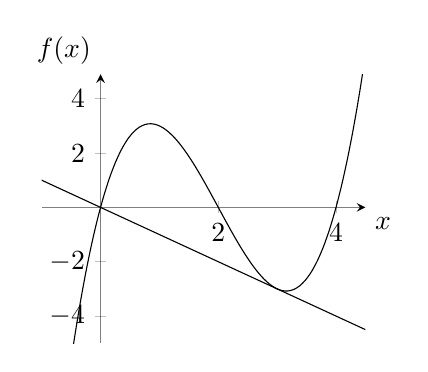
\begin{tikzpicture}
		\begin{axis}[scale=.6,draw opacity =.5,samples=100,smooth, 
		  axis x line=center, % no box around the plot, only x and y axis
		  axis y line=center, % the * suppresses the arrow tips
		  ylabel = {$f(x)$},
		  xlabel = {$x$},
		  xlabel style={below right},
		  ylabel style={above left},
		  xmin=-1,xmax=4,ymin=-5,ymax=4,
		  enlargelimits=upper] % extend the axes a bit to the right and top
		  \addplot[black,opacity=1]{x^3-6*x^2+8*x};
		  \addplot[black,opacity=1]{-x};
		\end{axis}
	    \end{tikzpicture}
	    \end{center}
	    \vspace{.5cm}
	    Primero calculemos la derivada de la recta y la curva, respectivamente
	    $$y'=-1,\qquad y_0'=3x^2-12x+8$$
	    Luego igualando estas ecuaciones obtenemos
	    $$y_1=3x^2-12x+8=-1\quad \Rightarrow \quad  x_1 = 3;\quad x_2=1.$$
	    Luego, para que la linea sea tangente a la curva, el punto debe estar en la curva $y_0=x^3-6x^2+8x$ como sigue,
	    \begin{itemize}
		\item Para $x_1=3$, se tiene $y(3)=-3=-x$ por lo que $y=-x$ es tangente a la curva en $(3,-3)$.\\
		\item Para $x_2=1$, se tiene $y(1)=1\neq -x$ por lo que $x_2$ no es tangente a la curva.\\
	    \end{itemize}
	    Esta linea tangente también corta la curva en $(0,0)$.\\\\

    %--------------------8.
    \item Dibujar la gráfica de la función cúbica $f(x)=x-x^3$ en el intervalo cerrado $-2\leq x\leq 2$. Hallar las constantes $m$ y $b$ de modo que la recta $y=mx+b$ sea tangente a la gráfica de $f$ en el punto $(-1,0)$. Una segunda recta que pasa por $(-1,0)$ es también tangente a la gráfica de $f$ en el punto $(a,c)$. Determinar las coordenadas $a$ y $c$.\\\\
	Respuesta.-\; 
	    \begin{center}
		\begin{tikzpicture}
		\begin{axis}[scale=.6,draw opacity =.5,samples=100,smooth, 
		  axis x line=center, % no box around the plot, only x and y axis
		  axis y line=center, % the * suppresses the arrow tips
		  ylabel = {$f(x)$},
		  xlabel = {$x$},
		  xlabel style={below right},
		  ylabel style={above left},
		  xmin=-2,xmax=2,ymin=-7,ymax=7,
		  enlargelimits=upper] % extend the axes a bit to the right and top
		  \addplot[black,opacity=1]{x-x^3};
		\end{axis}
	    \end{tikzpicture}
	    \end{center}
	    \vspace{.5cm}
	    Sea $f'(x)=1-3x^2$, entonce la tangente de la linea en el punto $(-1,0)$ será
	    $$f'(-1)=1-3(-1)^2 = -2 \quad \Rightarrow \quad m=-2.$$
	    de donde $b$ estará dado por,
	    $$y=mx+b\quad \Rightarrow \quad 0=-2(-1)+b \quad \Rightarrow \quad b=-2.$$
	    Por lo tanto 
	    $$y=-2x-2.$$
	    Después, supongamos otra linea tangente $y_1=m_1x+b_1$ a $f$ en el punto $(a,c)$ con pendiente 
	    $$f'(a)=1-3a^2=m_1$$
	    sabiendo que esta recta pasa por $(-1,0)$, entonces 
	    $$y_1(1)=0\quad \Rightarrow \quad (1-3a^2)(-1)+b_1=0\quad \Rightarrow \quad b_1=1-3a^2$$
	    Por lo que la recta $y_1$ es de la forma,
	    $$y_1=(1-3a^2)x+(1-3a^2).$$
	    Por último, dado que el punto $(a,c)$ está tanto en esta linea $y_1$ como en la curva $f$ tenemos
	    $$f(a)=c\quad \Rightarrow \quad a-a^3=c$$
	    $$\mbox{y}\qquad$$ 
	    $$y_1(a)=c\quad \Rightarrow \quad (1-3a^2)a+(1-3a^2)=c.$$
	    Igualando $c$ se tiene,
	    $$a-a^3=(1-3a^2)a+(1-3a^2) \quad \Rightarrow\quad 2a^3+3a^2-1=0 \quad \Rightarrow \quad 2a=\dfrac{1}{2}.$$
	    Ya que $a-a^3=c$ entonces $c=\dfrac{3}{8}.$ Así, el otro punto tangente está dado por $\left(\frac{1}{2},\frac{3}{8}\right).$\\\\

    %--------------------9.
    \item Una función $f$ está definida del modo siguiente:
    $$f(x)=\left\{\begin{array}{rcl}
	    \dfrac{1}{|x|}&\mbox{si}&|x|>c,\\\\
	    a+bx^2 &\mbox{si}&|x|\leq c.\\\\
    \end{array}\right.$$
    Hallar los valores de $a$ y $b$ (en función de $c$) tales que $f'(c)$ exista.\\\\
	Respuesta.-\; Sabemos que la derivada $f'(c)$ existe si y sólo si
	$$\lim_{h\to 0}\dfrac{f(c+h)-f(c)}{h}$$
	Existe. También sabemos que el límite existe si
	$$\lim_{h\to 0^+}\dfrac{f(c+h)-f(c)}{h} = \lim_{h\to 0^-}\dfrac{f(c+h)-f(c)}{h}.$$
	Por lo que si tomamos $c$ y nos acercamos a $ax+b$ desde la derecha, a $x^2$ desde la izquierda y tomando a $f(c)=c^2$, entonces 
	$$\begin{array}{rcl}
	    \lim\limits_{h\to 0^+} \dfrac{f(c+h)-f(c)}{h} &=& \lim\limits_{h\to 0^-} \dfrac{f(c+h)-f(c)}{h} \\\\
	    \lim\limits_{h\to 0^+} \dfrac{a(c+h)+b-c^2}{h} &=& \lim\limits_{h\to 0^-} \dfrac{(c+h)^2-c^2}{h} \\\\
	    \lim\limits_{h\to 0^+} \dfrac{ac+b-c^2}{h} + a &=& 2c.\\\\
	\end{array}$$
	Dado que $ac+b-c^2$ es una constante, entonces $\lim\limits_{h\to 0^+}\dfrac{ac+b-c^2}{h} = 0.$ Por lo que nos queda la ecuación 
	$$a=2c.$$
	Ahora dado que $\lim\limits_{h\to 0^+}\dfrac{ac+b-c^2}{h} = 0$, entonces
	$$ac+b-c^2=0 \quad \Rightarrow \quad b=-c^2.$$\\

    %--------------------10.
    \item Resolver el ejercicio 9 cuando $f$ es:
    $$f(x)=\left\{\begin{array}{lcl}
	    \dfrac{1}{|x|}&\mbox{si}&|x|>c,\\\\
	    a+bx^2 &\mbox{si}&|x|\leq c.\\
    \end{array}\right.$$\\
	Respuesta.-\; Supongamos que $c>0$ de lo contrario $f(x)=\dfrac{1}{|x|}$ para todo $x$. Entonces, existe la derivada para todo los valores de las constantes de $a$ y $b$. Luego sabemos que si una función tiene derivada en un punto $x$, entonces también es continua en $x$, por lo tanto la función $f$ es continua en $c$, así,\\
	$$\begin{array}{rcl}
	    \lim\limits_{x\to c^+}f(x)&=&\lim\limits_{x\to c^-}f(x)\\\\
	    \lim\limits_{x\to c^+}\dfrac{1}{|x|}&=&\lim\limits_{x\to c^-}a+bx^2\\\\
	    \dfrac{1}{c}&=&a+bc^2\\\\
			ac+bc^3&=&1\\\\
	\end{array}$$
	por otro lado,
	$$\begin{array}{rcl}
	    \lim\limits_{x\to 0^+}f(x)&=&\lim\limits_{x\to 0^-}f(x)\\\\
	    \lim\limits_{x\to 0^+}\dfrac{\frac{1}{|c+h|}-a+bc^2}{h}&=&\lim\limits_{x\to 0^-}\dfrac{a+b(c+h)^2-(a+bc^2)}{h}\\\\
	    \lim\limits_{x\to 0^+}\dfrac{\frac{1}{c+h}-a+bc^2}{h}\cdot \dfrac{c+h}{c+h}&=&\lim\limits_{x\to 0^-}\dfrac{2bch+bh^2}{h}\\\\
	    \lim\limits_{x\to 0^+}\dfrac{1-ac-bc^3-ah-bc^2h}{h(c+h)}&=&\lim\limits_{x\to 0^-}\dfrac{h(2bc+bh)}{h}\\\\
	    \lim\limits_{x\to 0^+}\dfrac{ac+bx^3-ac-bc^3-ah-bc^2h}{h}&=&\lim\limits_{x\to 0^-}2bc+bh\\\\
	    \lim\limits_{x\to 0^+}\dfrac{-h(a+bc^2)}{h(c+h)}&=&2bc+\lim\limits_{x\to 0^-}bh\\\\
	    \lim\limits_{x\to 0^+}-\dfrac{a+bc^2}{c+h}&=&2bc.\\\\
	    -\dfrac{a+bc^2}{c}&=&2bc.\\
	\end{array}$$
	Por último resolvemos las dos ecuaciones anteriores:
	$$\left\{\begin{array}{rcl}
		-\dfrac{a+bc^2}{c}&=&2bc\\\\
			   ac+bc^3&=&1\\
	\end{array}\right.
	\quad \Rightarrow \quad 
	\left\{\begin{array}{rcl}
		b &=& -\dfrac{1}{2c^3}\\\\
		a &=& -\dfrac{3}{2c}\\
	    \end{array}\right.$$\\\\

    %--------------------11.
    \item Resolver el ejercicio 9 cuando $f$ es:
    $$f(x)=\left\{\begin{array}{lcl}
	\sen x &\mbox{si}&x\leq c\\\\
	ax+b &\mbox{si}&x>c.\\
    \end{array}\right.$$\\\\
	Respuesta.-\; Sabemos que $f'(c)$ existe si y sólo si 
	$$\lim_{h\to 0}\dfrac{f(c+h)-f(c)}{h}$$
	Existe. También sabemos que el límite existe si y sólo si los dos límites unilaterales existen y son iguales, es decir
	$$\lim_{h\to 0^+}\dfrac{f(c+h)-f(c)}{h}=\lim_{h\to 0^-}\dfrac{f(c+h)-f(c)}{h}$$
	Por lo tanto usando la definición de $f$ tenemos,
	$$\begin{array}{rcl}
	    \lim\limits_{h\to 0^+} \dfrac{a(c+h)+b-\sen c}{h} &=& \lim\limits_{h\to 0^-} \dfrac{\sen (c+h)-\sen c}{h} \\\\
	    \lim\limits_{h\to 0^+} \left(\dfrac{ac + b-\sen c}{h}\right)+a &=& \lim\limits_{h\to 0^-} \dfrac{\sen c \cos h + \sen h \cos c - \sen c}{h}\\\\
	    \lim\limits_{h\to 0^+} \left(\dfrac{ac + b-\sen c}{h}\right)+a &=& \lim\limits_{h\to 0^-} \left[\dfrac{\sen c ( \cos h -1)}{h}\right] + \cos c \\\\
	\end{array}$$

	Al simplificar el lado derecho usamos el hecho de que $\lim\limits_{h\to 0}\dfrac{\sen h}{h}=1$. Además para que existe el límite por el lado izquierdo debemos tener $ac+b-\sen c = 0$ de lo contrario el límite divergirá como $h\to 0$. Ahora, para la expresión de la derecha, vemos que el límite tiende a $0$. Eso se puede ver ya que 
	$$\lim_{h\to 0^-}\dfrac{\sen c(\cos h - 1)}{h}=\sen c \lim_{h\to c^-}\dfrac{\cos h - 1}{h} = \sen c \lim_{h\to c^-}\dfrac{\cos(0+h)-\cos 0}{h}$$
	Pero este límite es la derivada de $\cos x$ en $x=0$. Luego ya que $(\cos x)'=-\sen x$ y $\sen 0 =0$ el termino tiende a $0$. Por lo tanto
	$$\lim\limits_{h\to 0^+} \left(\dfrac{ac + b-\sen c}{h}\right)+a = \lim\limits_{h\to 0^-} \left[\dfrac{\sen c ( \cos h -1)}{h}\right] + \cos c \quad \Rightarrow \quad a=\cos c.$$
	Así, dado que $ac+b-\sen c=0$ entonces 
	$$b=\sen c - c\cos c.$$\\

    %--------------------12.
    \item Si $f(x)=\dfrac{1-\sqrt{x}}{1+\sqrt{x}}$ para $x>0$, hallar fórmulas para $Df(x),\; D^2f(x)$ y $D^3f(x)$.\\\\
	Respuesta.- \; La fórmula para $Df(x)$ es:
	$$Df(x)=\dfrac{(1+\sqrt{x})\cdot \dfrac{-1}{2\sqrt{x}}- (1-\sqrt{x})\cdot \dfrac{1}{2\sqrt{x}}}{(1+\sqrt{x})^2} = \dfrac{\dfrac{1}{2}-\dfrac{1}{2}-\dfrac{1}{2\sqrt{x}}-\dfrac{1}{2\sqrt{x}}}{(1+\sqrt{x})^2}=\dfrac{-\dfrac{2}{2\sqrt{x}}}{(1+\sqrt{x})^2} =\dfrac{-1}{\sqrt{x}(1+\sqrt{x})^2}.$$

	Para $D^2f(x)$,

	$$D^2f(x)=\dfrac{\dfrac{1}{2\sqrt{x}}(1+\sqrt{x})^2+2\sqrt{x}(1+\sqrt{x})\dfrac{1}{2\sqrt{x}}}{x(1+\sqrt{x})^4} = \dfrac{1+3\sqrt{x}}{2(x+\sqrt{x})^3}.$$

	Por último para $D^3f(x)$,

	$$D^3f(x)=\dfrac{\dfrac{3}{2\sqrt{x}}\cdot 2(x+\sqrt{x})^3-6(1+3\sqrt{x})(x+\sqrt{x})^2\left(1+\dfrac{1}{2\sqrt{x}}\right)}{4(x+\sqrt{x})^6}=- \dfrac{3(1+4\sqrt{x}+5x)}{4\left[\sqrt{x}(x+\sqrt{x})^4\right]}.$$\\

    %--------------------13.
    \item Existe un polinomio $P(x)=ax^3+bx^2+cx+d$ tal que $P(0)=P(1)=-2,\; P'(0)=-1$ y $P''(0)=10.$Calcular $a,b,c,d.$\\\\
	Respuesta.-\; Primeramente calculamos la primera y segunda derivada de $P(x)$:
	$$P'(x)=ax^3+bx^2+cx+d,\qquad P''(x)=6ax+2b.$$
	De donde 
	$$P''(0)=6\cdot a\cdot 0+2b=10\quad \Rightarrow \quad b=5.$$
	$$\mbox{y}$$
	$$P'(0)=3\cdot a\cdot 0^2+2\cdot b \cdot 0 + c = -1 \quad \Rightarrow \quad c=-1.$$

	Luego calculamos $d$ y $a$ de la siguiente manera:
	$$P(0)=a\cdot 0^3+5\cdot 0^2-0+d=-2\quad \Rightarrow \quad d=-2.$$

	$$P(1)=a\cdot 1^3+5\cdot 1^2-1-2=-2\quad \Rightarrow \quad a=-4.$$

	Por lo tanto,
	$$a=-4,\quad b=5,\quad c=-1,\quad d=-2.$$\\

    %--------------------14.
    \item Dos funciones $f$ y $g$ admiten primera y segunda derivada en $0$ y satisfacen las relaciones 
	$$f(0)=\dfrac{2}{g(0)},\quad f'(0)=2g'(0)=4g(0),\quad g''(0)=5f''(0)=6f(0)=3.$$\\

	\begin{enumerate}[a)]

	    %---------- a)
	    \item Póngase $h(x)=\dfrac{f(x)}{g(x)}$, y calcular $h'(0).$\\\\
		Respuesta.-\; Usando la regla de derivada se tiene,
		$$h(x)=\dfrac{f(x)}{g(x)}\quad \Rightarrow \quad h'(x)=\dfrac{f'(x)-g(x)-f(x)g'(x)}{g^2(x)}.$$
		de donde sustituyendo obtenemos,
		$$\begin{array}{rcccl}
		    h'(0)&=&\dfrac{f'(0)g(0)-f(0)g'(0)}{g^2(0)}&=&\dfrac{4g^2(0)-f(0)g'(0)-\frac{2}{g(0)}2g(0)}{g^2(0)}\\\\
			 &=&\dfrac{4g^2(0)}{g^2(0)}-\dfrac{4}{g^2(0)} &=& 4-\dfrac{4}{\frac{4}{f^2(0)}}\\\\
			 &=& 4-\dfrac{4}{\frac{4}{\left(\frac{1}{2}\right)^2}}&=&\dfrac{15}{4}
		\end{array}$$
		\vspace{.7cm}

	    %---------- b)
	    \item Póngase $k(x)=f(x)g(x)\sen x$, y calcular $k'(0).$\\\\
		Respuesta.-\; Usando la propiedad del producto derivamos como sigue,\\
		$$k'(x)=f'(x)g'(x)\sen x + f(x)g'(x)\sen x + f(x)g(x)\cos x$$
		Luego evaluamos en $0$,
		$$k'(0)=f'(0)g'(0)\sen 0 + f(0)g'(0)\sen 0 + f(0)g(0)\cos 0 = f(0)g(0)=2.$$\\

	    %---------- c)
	    \item Calcular el límite de $\dfrac{g'(x)}{f'(x)}$ cuando $x\to 0$.\\\\
		Respuesta.-\; Sabemos que si $f$ y $g$ son diferenciables entonces son continuos, esto significa
		$$\lim_{x\to 0}f'(x)=f'(0)\quad \mbox{y}\quad \lim_{x\to 0}g'(x)=g'(0)$$
		Además $f'(0)\neq 0$ ya que $f'(0)=4g(0)$ y $g(0)=\dfrac{2}{f(0)}=\dfrac{2}{\frac{1}{2}}=4$, por lo tanto
		$$\lim_{x\to 0}\dfrac{g'(x)}{f'(x)}=\dfrac{\lim\limits_{x\to 0}g'(x)}{\lim\limits_{x\to 0}f'(x)}=\dfrac{g'(0)}{f'(0)}=\dfrac{g'(0)}{2g'(0)}=\dfrac{1}{2}.$$\\

	\end{enumerate}

    %--------------------15.
    \item Supóngase que existe la derivada $f'(a)$. Indicar cuáles de las desigualdades siguientes son ciertas y cuáles falsas. Expresar el fundamento de la decisión en cada caso.

	\begin{enumerate}[(a)]

	    %---------- (a)
	    \item $f'(a)=\lim\limits_{h\to a}\dfrac{f(h)-f(a)}{h-a}$.\\\\
		Respuesta.-\; Sea $j=h-a$ entonces
		$$\lim_{h\to a}\dfrac{f(h)-f(a)}{h-a}=\lim_{h\to a}\dfrac{f(a-a+h)-f(a)}{h-a}=\lim_{j\to 0}\dfrac{f(a+j)-f(a)}{j}=f'(a).$$
		Por lo que $f'(a)$ es verdadera.\\\\

	    %---------- (b)
	    \item $f'(a)=\lim\limits_{h\to 0}\dfrac{f(a)-f(a+h)}{h}$.\\\\
		Respuesta.-\; Sea $j=-h$, entonces
		$$\lim_{h\to 0}\dfrac{f(a)-f(a-h)}{h}=\lim_{h\to a}\dfrac{f(a)-f(a+j)}{-j}=\lim_{t\to 0}\dfrac{f(a+j)-f(a)}{j}.$$\\
		Por lo tanto $f'(a)$ es verdadera.\\\\

	    %---------- (c)
	    \item $f'(a)=\lim\limits_{t\to 0}\dfrac{f(a+2t)-f(a)}{t}$.\\\\
		Respuesta.-\; Sea $j=2t$, entonces
		$$\lim_{t\to 0}\dfrac{f(a+2t)-f(a)}{t}=\lim_{t\to 0}=2\cdot\dfrac{f(a+2t)-f(a)}{2t}=2\cdot \lim_{t\to 0}\dfrac{f(a+j)-f(a)}{j}=2f'(a)\neq f'(a).$$\\
		Por lo tanto $f'(a)$ es falsa.\\\\

	    %---------- (d)
	    \item $f'(a)=\lim\limits_{t\to 0}\dfrac{f(a+2t)-f(a+t)}{2t}$.\\\\
		Respuesta.-\; Sea $j=2t$, entonces
		$$\begin{array}{rcl}
		    \lim\limits_{t\to 0}\dfrac{f(a+2t)-f(a+t)}{2t}&=&\lim\limits_{t\to 0}\dfrac{f(a+2t)-f(a+t)+f(a)-f(a)}{2t}\\\\
						  &=&\lim\limits_{t\to 0}\dfrac{f(a+2t)-f(a)}{2t}-\lim\limits_{t\to 0}\dfrac{f(a+t)-f(a)}{2t}\\\\
						  &=&\lim\limits_{t\to 0}\dfrac{f(a+j)-f(a)}{j}-\dfrac{1}{2}\cdot \lim\limits_{t\to 0}\dfrac{f(a+t)-f(a)}{t}\\\\
						  &=&f'(a)-\dfrac{1}{2}f'(a)\\\\
						  &=&\dfrac{1}{2}f'(a)\neq f'(a).\\\\
		\end{array}$$
		Por lo tanto $f'(a)$ es falsa.\\\\

	\end{enumerate}

    %--------------------16.
    \item Supóngase que en lugar de la definición usual de derivada $Df(x)$ se define una nueva clase de derivada $D^*f(x)$ por fórmula:
	$$D^*f(x)=\lim_{h\to 0}\dfrac{f^2(x+h)-f^2(x)}{h},$$
	donde $f^2(x)$ significa $[f(x)]^2.$\\

	\begin{enumerate}[(a)]

	    %---------- (a)
	    \item Hallar fórmulas para calcular la derivada $D^*$ de una suma, diferencia, producto y cociente.\\\\
		Respuesta.-\; Sea $f$ y $g$. Para la suma se tiene,
		$$\begin{array}{rcl}
		    D^*\left[f(x)+g(x)\right]&=&\lim\limits_{h\to 0}\dfrac{\left[f(x+h)+g(x+h)\right]^2-\left[f(x)+g(x)\right]^2}{h}\\\\
					     &=&\lim\limits_{h\to 0}\dfrac{f^2(x+h)+2f(x+h)(x+h)+g^2(x+h)-f^2(x)-2f(x)g(x)-g^2(x)}{h}\\\\
					     &=&\lim\limits_{h\to 0}\left[\dfrac{f^2(x+h)-f^2(x)}{h}\right]+2\lim\limits_{h\to 0}\left[\dfrac{f(x+h)g(x+h)-f(x)g(x)}{h}\right]\\\\
					     &+&\lim\limits_{h\to 0}\left[\dfrac{g^2(x+h)-g^2(x)}{h}\right]\\\\
					     &=&D^*f(x)+d^*g(x)+2\lim\limits_{h\to 0}\left[\dfrac{f(x+h)g(x+h)-f(x)g(x)}{h}\right].\\\\
		\end{array}$$
		Luego multiplicamos el límite anterior por $\dfrac{f(x+h)g(x+h)+f(x)g(x)}{f(x+h)g(x+h)+f(x)g(x)}$, de donde
		$$\begin{array}{rcl}
		    &=&D^*f(x)+f^*g(x)+2\lim\limits_{h\to 0}\left[\dfrac{f(x+h)g(x+h)-f(x)g(x)}{h}\cdot \dfrac{f(x+h)g(x+h)+f(x)g(x)}{f(x+h)g(x+h)+f(x)g(x)}\right]\\\\
		    &=&D^*f(x)+D^*g(x)+2\lim\limits_{h\to 0}\left[\dfrac{f^2(x+h)g^2(x+h)-f^2(x)g^2(x)}{h\left(f(x+h)g(x+h)+f(x)g(x)\right)}\right]\\\\
		    &=&D^*f(x)+D^*g(x)+\dfrac{1}{f(x)g(x)}\lim\limits_{h\to 0}\dfrac{\left[f(x+h)g(x+h)\right]-\left[f(x)g(x)\right]^2}{h}.\\\\
		\end{array}$$
		Ahora, para el límite restante, usamos la regla del producto para la derivada en esta definición alternativa, que derivamos a continuación. (Este último límite es $D^* (f(x)g(x))$. Luego derivamos que $D^* (f(x)g(x)) = g^2 D^*f + f^2 D^* g)$. Por lo tanto,
		$$\begin{array}{rcl}
		    D^*\left[f(x)+g(x)\right] &=&D^*f(x)+D^*g(x)+\dfrac{1}{f(x)g(x)}\lim\limits_{h\to 0}\dfrac{\left[f(x+h)g(x+h)\right]-\left[f(x)g(x)\right]^2}{h}.\\\\
					      &=&D^*f(x)+D^*g(x)+\dfrac{1}{f(x)g(x)}\left[g^2(x)D^*f(x)+f^2(x)D^*g(x)\right]\\\\
					      &=&D^*f(x)+D^*g(x)+\dfrac{g(x)}{f(x)}D^*f(x)+\dfrac{f(x)}{g(x)}D^*g(x)\\\\
					      &=&\left(1+\dfrac{g(x)}{f(x)}\right)D^*f(x)+\left(1+\dfrac{f(x)}{g(x)}\right)D^*g(x)\\\\
		\end{array}$$

		Para la diferencia se sigue similar a la suma,

		$$D^*\left[f(x)-g(x)\right]=\left(1-\dfrac{g(x)}{f(x)}\right)D^*f(x)+\left(1-\dfrac{f(x)}{g(x)}\right)D^*g(x)$$

		Para el producto tenemos,

		$$\begin{array}{rcl}
		    D^*\left[f(x)g(x)\right] &=&\lim\limits_{h\to 0}\dfrac{\left[f(x+h)g(x+h)\right]^2-\left[f(x)g(x)\right]^2}{h}\\\\ 
					     &=&\lim\limits_{h\to 0}\dfrac{f^2(x+h)g^2(x+h)-f^2(x)g^2(x)}{h}\\\\
					     &=&\lim\limits_{h\to 0}\dfrac{f^2(x+h)g^2(x+h)-f^2(x)g^2(x)+f^2(x+h)g^2(x)-f^2(x+h)g^2(x)}{h}\\\\
					     &=&\lim\limits_{h\to 0}\left[g^2(x)\dfrac{f^2(x+h)-f^2(x)}{h}\right]+\lim\limits_{h\to 0}\left[f^2(x+h)\dfrac{g^2(x+h)-g^2(x)}{h}\right]\\\\
					     &=&g^2(x)D^*f+f^2(x)D^*g.\\\\

		\end{array}$$

		Por último para el cociente tenemos,

		$$\begin{array}{rcl}
		    D^*\left[\dfrac{f(x)}{g(x)}\right]&=&\lim\limits_{h\to 0}\dfrac{\frac{f^2(x+h)}{g^2(x+h)}-\frac{f^2(x)}{g^2(x)}}{h}\\\\
						      &=&\lim\limits_{h\to 0}\left[\dfrac{g^2(x)f^2(x+h)-f^2(x)g^2(x+h)}{h\cdot g^2(x+h)g^2(x)}\right]\\\\
						      &=&\dfrac{1}{g^4(x)}\lim\limits_{h\to 0}\left[\dfrac{g^2(x)f^2(x+h)-f^2(x)g^2(x+h)+g^2(x)f^2(x)-g^2(x)f^2(x)}{h}\right]\\\\
						      &=&\dfrac{1}{g^4(x)}\lim\limits_{h\to 0}\left[g^2(x)\dfrac{f^2(x+h)-f^2(x)}{h}-f^2(x)\dfrac{g^2(x+h)-g^2(x)}{h}\right]\\\\
						      &=&\dfrac{g^2D^*f-f^2D^*g}{g^4}\\\\
		\end{array}$$



	    %---------- (b)
	    \item Expresar $D^*f(x)$ en función de $Df(x)$.\\\\
		Respuesta.-\; Usaremos la idea de $\lim_{h \to 0} f(x+h) = f(x)$, y que $f(x)$ es una constante en $h$, por lo que podemos sacar el límite. 
		$$D^*f(x)=\lim_{h\to 0}\dfrac{f^2(x+h)-f^28x)}{h}=\lim_{h\to 0}\dfrac{\left[f(x+h)+f(x)\right]\left[f(x+h)-f(x)\right]}{h}=2f(x)\cdot Df(x).$$\\


	    %---------- (c)
	    \item ¿Para qué funciones es $D^*f=Df$?.\\\\
		Respuesta.-\; Para encontrar la función $f$ tal que $Df=D^*f$ igualamos las dos expresiones y resolvemos $f$ usando $D^*f=2D f$, como sigue
		$$Df=D^*f\quad \Rightarrow \quad Df=2f(x)Df\quad \Rightarrow \quad Df=0\; \mbox{o}\; 2f(x)=1.$$
		En cualquier caso tenemos $f(x)=c$ para alguna constante $c$.\\\\

	\end{enumerate}

\end{enumerate}


\section{Regla de la cadena para la derivación de funciones compuestas}
